\chapter{Установка NS3}
\section{Определение NS3}
NS-3, также известный как Network Simulator 3~\cite{ns3}, --- это сетевой
симулятор с открытым исходным кодом, используемый для исследований и
разработок в области компьютерных сетей. Он используется для
моделирования, имитации и оценки поведения коммуникационных сетей,
таких как проводные сети, беспроводные сети, сенсорные сети, сети
межсетевого взаимодействия и т.д.

NS-3 предлагает широкий набор функций для моделирования различных аспектов сетей, включая: 
\begin{itemize}
    \item моделирование протоколов связи;
    \item управление каналами передачи данных;
    \item управление трафиком;
    \item моделирование мобильных объектов;
    \item моделирование помех и т.д.
\end{itemize}


NS-3 позволяет исследователям и разработчикам тестировать и проверять
новые идеи, сравнивать эффективность различных стратегий и
анализировать поведение сетей в конкретных сценариях.

NS-3 написан на C++ и предоставляет интерфейсы программирования (API),
которые позволяют пользователям создавать собственные сценарии
моделирования путем написания кода. NS-3 широко используется в
академических и промышленных кругах для исследования сетей, обучения,
разработки протоколов и оценки производительности.

\section{Возможности NS-3}

Моделирование протоколов: NS-3 предлагает библиотеку уже существующих
моделей протоколов для моделирования различных коммуникационных
протоколов, таких как TCP/IP, UDP, IPv4, IPv6, OSPF, BGP и др. Эти
модели позволяют исследователям оценить производительность этих
протоколов в различных сценариях.

Проводные и беспроводные сети: NS-3 поддерживает моделирование как
проводных, так и беспроводных сетей, включая сети Ad Hoc, сенсорные
сети, сотовые сети, сети Wi-Fi и так далее. Это позволяет
анализировать производительность сети в различных конфигурациях и
условиях.

Моделирование мобильности: NS-3 предлагает модели мобильности для
моделирования перемещения узлов в сети. Они включают модели случайной
мобильности, броуновского движения, движения, основанного на реальных
следах, и т.д. Эти модели можно использовать для оценки
производительности протоколов маршрутизации и управления мобильностью.

Интерференция и распространение волн: NS-3 моделирует интерференцию
между узлами в беспроводной сети. Она также учитывает эффекты
распространения волн, такие как ослабление сигнала, отражение,
рассеяние и так далее. Это позволяет оценить работу протоколов в
реалистичных условиях.

Программирование и настройка: NS-3 предлагает интерфейс
программирования (API) на C++, позволяющий пользователям настраивать и
расширять функциональность платформы. Пользователи могут создавать
собственные модели протоколов, сценарии моделирования и анализа
результатов.

Интеграция с другими инструментами: NS-3 может быть интегрирована с
другими инструментами моделирования и визуализации, такими как
Wireshark, для захвата и анализа пакетов, обменивающихся в
моделируемой сети. Это позволяет проводить углубленный анализ
поведения сети и протоколов.

NS-3 --- это мощная и гибкая платформа для моделирования сетей,
предлагающая расширенные возможности для исследований, разработок и
оценки производительности компьютерных сетей.

\section{Установка NS3}
Установка NS-3 может быть сложным процессом. 
Точные шаги могут отличаться в зависимости от используемой операционной
системы. Следующие инструкции основаны на установке под ОС Linux.

Сначала необходимо убедиться, что операционной системе установлены
необходимые зависимости, такие как GCC, Python, Git и т.д. Полный
список необходимых условий для  операционной системы можно найти
в документации NS-3.

Затем необходимо загрузить (клонировать) репозиторий NS-3 с GitHub:
\begin{verbatim}
    git clone https://github.com/nsnam/ns-3-dev-git
\end{verbatim}

Для конфигурации NS-3 необходимо перейти в каталог:
\begin{verbatim}
    cd ns-3-dev-git
\end{verbatim}
и запустить сценарий конфигурации для обнаружения и настройки зависимостей:
\begin{verbatim}
    ./ns3 configure --examples
\end{verbatim}

После завершения конфигурации необходимо выполнить следующую команду для компиляции NS-3:
\begin{verbatim}
    ./ns3 build
\end{verbatim}

При этом следует заменить значение «3.28» на версию NS3, которая была
скачана. Чтобы убедиться, что NS3 установлен правильно, требуется
выполнить следующую команду:

\begin{verbatim}
    ./ns3 --run first
\end{verbatim}

\begin{figure}[!h]
  \centering
  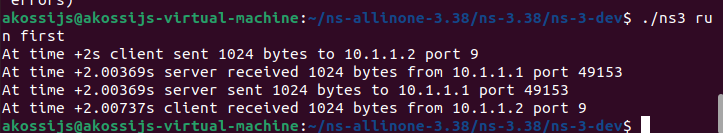
\includegraphics[width=0.9\linewidth]{image/003.PNG}
  \caption{Первый запуск NS-3}
  \label{fig:ns3:1.1}
\end{figure}

\section{Запуск NS-3 с VANET}

Интеграция моделирования VANET в NS3 позволяет изучать поведение
автомобильных сетей в различных сценариях. Это может включать
моделирование мобильности транспортных средств, распространения
радиоволн, подключения к сети, управления ресурсами и других аспектов,
связанных с VANET.

Используя NS3 с VANET, мы можем оценить производительность протоколов
связи, протестировать новые стратегии маршрутизации, изучить алгоритмы
безопасности, проанализировать влияние различных факторов на
производительность сети и так далее. Это позволяет проводить
виртуальные эксперименты до их развертывания в реальной среде, что
зачастую является дорогостоящим и сложным.

Для запуска примера модели с VANET необходимо перейти в каталог
\verb|scratch| в ns3, используя следующую команду:
\begin{verbatim}
    cd /home/akossijs/ns-allinone 3.38/ns-3.38/ns-3.38-dev/scratch
\end{verbatim}
Затем запустить следующую команду:
\begin{verbatim}
    ./ns3 run vanet-routing-comapare
\end{verbatim}

\begin{figure}[!h]
  \centering
  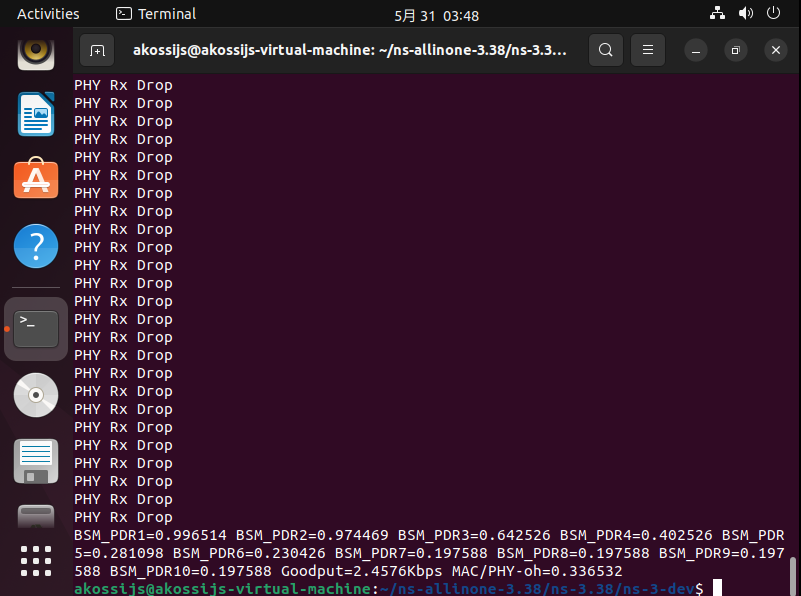
\includegraphics[width=0.9\linewidth]{image/004.PNG}
  \caption{Окончание  компиляции примера с VANET}
  \label{fig:ns3:1.2}
\end{figure}